\documentclass{article}

\def \lastexercisenumber {0}

% Hier befinden sich Pakete, die wir beinahe immer benutzen ...

\usepackage[utf8]{inputenc}

% Sprach-Paket:
\usepackage[ngerman]{babel}

% damit's nicht so, wie beim Grill aussieht:
\usepackage{fullpage}

% Mathematik:
\usepackage{amsmath, amssymb, amsfonts, amsthm}
\usepackage{bbm}
\usepackage{mathtools, mathdots}

% Makros mit mehereren Default-Argumenten:
\usepackage{twoopt}

% Anführungszeichen (Makro \Quote{}):
\usepackage{babel}

% if's für Makros:
\usepackage{xifthen}
\usepackage{etoolbox}

% tikz ist kein Zeichenprogramm (doch!):
\usepackage{tikz}

% bessere Aufzählungen:
\usepackage{enumitem}

% (bessere) Umgebung für Bilder:
\usepackage{graphicx, subfig, float}

% Umgebung für Code:
\usepackage{listings}

% Farben:
\usepackage{xcolor}

% Umgebung für "plain text":
\usepackage{verbatim}

% Umgebung für mehrerer Spalten:
\usepackage{multicol}

% "nette" Brüche
\usepackage{nicefrac}

% Spaltentypen verschiedener Dicke
\usepackage{tabularx}
\usepackage{makecell}

% Für Vektoren
\usepackage{esvect}

% (Web-)Links
\usepackage{hyperref}

% Zitieren & Literatur-Verzeichnis
\usepackage[style = authoryear]{biblatex}
\usepackage{csquotes}

% so ähnlich wie mathbb
%\usepackage{mathds}

% Keine Ahnung, was das macht ...
\usepackage{booktabs}
\usepackage{ngerman}
\usepackage{placeins}

% special letters:

\newcommand{\N}{\mathbb{N}}
\newcommand{\Z}{\mathbb{Z}}
\newcommand{\Q}{\mathbb{Q}}
\newcommand{\R}{\mathbb{R}}
\newcommand{\C}{\mathbb{C}}
\newcommand{\K}{\mathbb{K}}
\newcommand{\T}{\mathbb{T}}
\newcommand{\E}{\mathbb{E}}
\newcommand{\V}{\mathbb{V}}
\renewcommand{\S}{\mathbb{S}}
\renewcommand{\P}{\mathbb{P}}
\newcommand{\1}{\mathbbm{1}}

% quantors:

\newcommand{\Forall}{\forall \,}
\newcommand{\Exists}{\exists \,}
\newcommand{\ExistsOnlyOne}{\exists! \,}
\newcommand{\nExists}{\nexists \,}
\newcommand{\ForAlmostAll}{\forall^\infty \,}

% MISC symbols:

\newcommand{\landau}{{\scriptstyle \mathcal{O}}}
\newcommand{\Landau}{\mathcal{O}}


\newcommand{\eps}{\mathrm{eps}}

% graphics in a box:

\newcommandtwoopt
{\includegraphicsboxed}[3][][]
{
  \begin{figure}[!h]
    \begin{boxedin}
      \ifthenelse{\isempty{#1}}
      {
        \begin{center}
          \includegraphics[width = 0.75 \textwidth]{#3}
          \label{fig:#2}
        \end{center}
      }{
        \begin{center}
          \includegraphics[width = 0.75 \textwidth]{#3}
          \caption{#1}
          \label{fig:#2}
        \end{center}
      }
    \end{boxedin}
  \end{figure}
}

% braces:

\newcommand{\pbraces}[1]{{\left  ( #1 \right  )}}
\newcommand{\bbraces}[1]{{\left  [ #1 \right  ]}}
\newcommand{\Bbraces}[1]{{\left \{ #1 \right \}}}
\newcommand{\vbraces}[1]{{\left  | #1 \right  |}}
\newcommand{\Vbraces}[1]{{\left \| #1 \right \|}}
\newcommand{\abraces}[1]{{\left \langle #1 \right \rangle}}
\newcommand{\round}[1]{\bbraces{#1}}

\newcommand
{\floorbraces}[1]
{{\left \lfloor #1 \right \rfloor}}

\newcommand
{\ceilbraces} [1]
{{\left \lceil  #1 \right \rceil }}

% special functions:

\newcommand{\norm}  [2][]{\Vbraces{#2}_{#1}}
\newcommand{\diam}  [2][]{\mathrm{diam}_{#1} \: #2}
\newcommand{\diag}  [1]{\mathrm{diag} \: #1}
\newcommand{\dist}  [1]{\mathrm{dist} \: #1}
\newcommand{\mean}  [1]{\mathrm{mean} \: #1}
\newcommand{\erf}   [1]{\mathrm{erf} \: #1}
\newcommand{\id}    [1]{\mathrm{id} \: #1}
\newcommand{\sgn}   [1]{\mathrm{sgn} \: #1}
\newcommand{\supp}  [1]{\mathrm{supp} \: #1}
\newcommand{\arsinh}[1]{\mathrm{arsinh} \: #1}
\newcommand{\arcosh}[1]{\mathrm{arcosh} \: #1}
\newcommand{\artanh}[1]{\mathrm{artanh} \: #1}
\newcommand{\card}  [1]{\mathrm{card} \: #1}
\newcommand{\Span}  [1]{\mathrm{span} \: #1}
\newcommand{\Aut}   [1]{\mathrm{Aut} \: #1}
\newcommand{\End}   [1]{\mathrm{End} \: #1}
\newcommand{\ggT}   [1]{\mathrm{ggT} \: #1}
\newcommand{\kgV}   [1]{\mathrm{kgV} \: #1}
\newcommand{\ord}   [1]{\mathrm{ord} \: #1}
\newcommand{\grad}  [1]{\mathrm{grad} \: #1}
\newcommand{\ran}   [1]{\mathrm{ran} \: #1}
\newcommand{\graph} [1]{\mathrm{graph} \: #1}
\newcommand{\Inv}   [1]{\mathrm{Inv} \: #1}
\newcommand{\pv}    [1]{\mathrm{pv} \: #1}
\newcommand{\GL}    [1]{\mathrm{GL} \: #1}
\newcommand{\Mod}{\mathrm{Mod} \:}
\newcommand{\Th}{\mathrm{Th} \:}
\newcommand{\Char}{\mathrm{char}}
\newcommand{\At}{\mathrm{At}}
\newcommand{\Ob}{\mathrm{Ob}}
\newcommand{\Hom}{\mathrm{Hom}}
\newcommand{\orthogonal}[3][]{#2 ~\bot_{#1}~ #3}
\newcommand{\Rang}{\mathrm{Rang}}
\newcommand{\NIL}{\mathrm{NIL}}
\newcommand{\Res}{\mathrm{Res}}
\newcommand{\lxor}{\dot \lor}
\newcommand{\Div}{\mathrm{div} \:}
\newcommand{\meas}{\mathrm{meas} \:}

% fractions:

\newcommand{\Frac}[2]{\frac{1}{#1} \pbraces{#2}}
\newcommand{\nfrac}[2]{\nicefrac{#1}{#2}}

% derivatives & integrals:

\newcommandtwoopt
{\Int}[4][][]
{\int_{#1}^{#2} #3 ~\mathrm{d} #4}

\newcommandtwoopt
{\derivative}[3][][]
{
  \frac
  {\mathrm{d}^{#1} #2}
  {\mathrm{d} #3^{#1}}
}

\newcommandtwoopt
{\pderivative}[3][][]
{
  \frac
  {\partial^{#1} #2}
  {\partial #3^{#1}}
}

\newcommand
{\primeprime}
{{\prime \prime}}

\newcommand
{\primeprimeprime}
{{\prime \prime \prime}}

% Text:

\newcommand{\Quote}[1]{\glqq #1\grqq{}}
\newcommand{\Text}[1]{{\text{#1}}}
\newcommand{\fastueberall}{\text{f.ü.}}
\newcommand{\fastsicher}{\text{f.s.}}

% -------------------------------- %
% amsthm-stuff:

\theoremstyle{definition}

% numbered theorems
\newtheorem{theorem}{Satz}
\newtheorem{lemma}{Lemma}
\newtheorem{corollary}{Korollar}
\newtheorem{proposition}{Proposition}
\newtheorem{remark}{Bemerkung}
\newtheorem{definition}{Definition}
\newtheorem{example}{Beispiel}

% unnumbered theorems
\newtheorem*{theorem*}{Satz}
\newtheorem*{lemma*}{Lemma}
\newtheorem*{corollary*}{Korollar}
\newtheorem*{proposition*}{Proposition}
\newtheorem*{remark*}{Bemerkung}
\newtheorem*{definition*}{Definition}
\newtheorem*{example*}{Beispiel}

% Please define this stuff in project ("main.tex"):

% \def \lastexercisenumber {...}
% This will be 0 by default

% \setcounter{section}{...}
% This will be 0 by default
% and hence, completely ignored

\ifnum \thesection = 0
{\newtheorem{exercise}{Aufgabe}}
\else
{\newtheorem{exercise}{Aufgabe}[section]}
\fi

\ifdef
{\lastexercisenumber}
{\setcounter{exercise}{\lastexercisenumber}}

\newcommand{\solution}
{
    \renewcommand{\proofname}{Lösung}
    \renewcommand{\qedsymbol}{}
    \proof
}

\renewcommand{\proofname}{Beweis}

% -------------------------------- %
% environment zum einkasteln:

% dickere vertical lines
\newcolumntype
{x}
[1]
{!{\centering\arraybackslash\vrule width #1}}

% environment selbst (the big cheese)
\newenvironment
{boxedin}
{
  \begin{tabular}
  {
    x{1 pt}
    p{\textwidth}
    x{1 pt}
  }
  \Xhline
  {2 \arrayrulewidth}
}
{
  \\
  \Xhline{2 \arrayrulewidth}
  \end{tabular}
}

% -------------------------------- %
% MISC "Ein-Deutschungen"

\renewcommand
{\figurename}
{Abbildung}

\renewcommand
{\tablename}
{Tabelle}

% -------------------------------- %

% ---------------------------------------------------------------- %
% https://www.overleaf.com/learn/latex/Code_listing

\definecolor{codegreen} {rgb}{0, 0.6, 0}
\definecolor{codegray}    {rgb}{0.5, 0.5, 0.5}
\definecolor{codepurple}{rgb}{0.58, 0, 0.82}
\definecolor{backcolour}{rgb}{0.95, 0.95, 0.92}

\lstdefinestyle{overleaf}
{
    backgroundcolor = \color{backcolour},
    commentstyle = \color{codegreen},
    keywordstyle = \color{magenta},
    numberstyle = \tiny\color{codegray},
    stringstyle = \color{codepurple},
    basicstyle = \ttfamily \footnotesize,
    breakatwhitespace = false,
    breaklines = true,
    captionpos = b,
    keepspaces = true,
    numbers = left,
    numbersep = 5pt,
    showspaces = false,
    showstringspaces = false,
    showtabs = false,
    tabsize = 2
}

% ---------------------------------------------------------------- %
% https://en.wikibooks.org/wiki/LaTeX/Source_Code_Listings

\lstdefinestyle{customc}
{
    belowcaptionskip = 1 \baselineskip,
    breaklines = true,
    frame = L,
    xleftmargin = \parindent,
    language = C,
    showstringspaces = false,
    basicstyle = \footnotesize \ttfamily,
    keywordstyle = \bfseries \color{green!40!black},
    commentstyle = \itshape \color{purple!40!black},
    identifierstyle = \color{blue},
    stringstyle = \color{orange},
}

\lstdefinestyle{customasm}
{
    belowcaptionskip = 1 \baselineskip,
    frame = L,
    xleftmargin = \parindent,
    language = [x86masm] Assembler,
    basicstyle = \footnotesize\ttfamily,
    commentstyle = \itshape\color{purple!40!black},
}

% ---------------------------------------------------------------- %
% https://tex.stackexchange.com/questions/235731/listings-syntax-for-literate

\definecolor{maroon}        {cmyk}{0, 0.87, 0.68, 0.32}
\definecolor{halfgray}      {gray}{0.55}
\definecolor{ipython_frame} {RGB}{207, 207, 207}
\definecolor{ipython_bg}    {RGB}{247, 247, 247}
\definecolor{ipython_red}   {RGB}{186, 33, 33}
\definecolor{ipython_green} {RGB}{0, 128, 0}
\definecolor{ipython_cyan}  {RGB}{64, 128, 128}
\definecolor{ipython_purple}{RGB}{170, 34, 255}

\lstdefinestyle{stackexchangePython}
{
    breaklines = true,
    %
    extendedchars = true,
    literate =
    {á}{{\' a}} 1 {é}{{\' e}} 1 {í}{{\' i}} 1 {ó}{{\' o}} 1 {ú}{{\' u}} 1
    {Á}{{\' A}} 1 {É}{{\' E}} 1 {Í}{{\' I}} 1 {Ó}{{\' O}} 1 {Ú}{{\' U}} 1
    {à}{{\` a}} 1 {è}{{\` e}} 1 {ì}{{\` i}} 1 {ò}{{\` o}} 1 {ù}{{\` u}} 1
    {À}{{\` A}} 1 {È}{{\' E}} 1 {Ì}{{\` I}} 1 {Ò}{{\` O}} 1 {Ù}{{\` U}} 1
    {ä}{{\" a}} 1 {ë}{{\" e}} 1 {ï}{{\" i}} 1 {ö}{{\" o}} 1 {ü}{{\" u}} 1
    {Ä}{{\" A}} 1 {Ë}{{\" E}} 1 {Ï}{{\" I}} 1 {Ö}{{\" O}} 1 {Ü}{{\" U}} 1
    {â}{{\^ a}} 1 {ê}{{\^ e}} 1 {î}{{\^ i}} 1 {ô}{{\^ o}} 1 {û}{{\^ u}} 1
    {Â}{{\^ A}} 1 {Ê}{{\^ E}} 1 {Î}{{\^ I}} 1 {Ô}{{\^ O}} 1 {Û}{{\^ U}} 1
    {œ}{{\oe}}  1 {Œ}{{\OE}}  1 {æ}{{\ae}}  1 {Æ}{{\AE}}  1 {ß}{{\ss}}  1
    {ç}{{\c c}} 1 {Ç}{{\c C}} 1 {ø}{{\o}} 1 {å}{{\r a}} 1 {Å}{{\r A}} 1
    {€}{{\EUR}} 1 {£}{{\pounds}} 1
}


% Python definition (c) 1998 Michael Weber
% Additional definitions (2013) Alexis Dimitriadis
% modified by me (should not have empty lines)

\lstdefinelanguage{iPython}{
    morekeywords = {access, and, break, class, continue, def, del, elif, else, except, exec, finally, for, from, global, if, import, in, is, lambda, not, or, pass, print, raise, return, try, while}, %
    %
    % Built-ins
    morekeywords = [2]{abs, all, any, basestring, bin, bool, bytearray, callable, chr, classmethod, cmp, compile, complex, delattr, dict, dir, divmod, enumerate, eval, execfile, file, filter, float, format, frozenset, getattr, globals, hasattr, hash, help, hex, id, input, int, isinstance, issubclass, iter, len, list, locals, long, map, max, memoryview, min, next, object, oct, open, ord, pow, property, range, raw_input, reduce, reload, repr, reversed, round, set, setattr, slice, sorted, staticmethod, str, sum, super, tuple, type, unichr, unicode, vars, xrange, zip, apply, buffer, coerce, intern}, %
    %
    sensitive = true, %
    morecomment = [l] \#, %
    morestring = [b]', %
    morestring = [b]", %
    %
    morestring = [s]{'''}{'''}, % used for documentation text (mulitiline strings)
    morestring = [s]{"""}{"""}, % added by Philipp Matthias Hahn
    %
    morestring = [s]{r'}{'},     % `raw' strings
    morestring = [s]{r"}{"},     %
    morestring = [s]{r'''}{'''}, %
    morestring = [s]{r"""}{"""}, %
    morestring = [s]{u'}{'},     % unicode strings
    morestring = [s]{u"}{"},     %
    morestring = [s]{u'''}{'''}, %
    morestring = [s]{u"""}{"""}, %
    %
    % {replace}{replacement}{lenght of replace}
    % *{-}{-}{1} will not replace in comments and so on
    literate = 
    {á}{{\' a}} 1 {é}{{\' e}} 1 {í}{{\' i}} 1 {ó}{{\' o}} 1 {ú}{{\' u}} 1
    {Á}{{\' A}} 1 {É}{{\' E}} 1 {Í}{{\' I}} 1 {Ó}{{\' O}} 1 {Ú}{{\' U}} 1
    {à}{{\` a}} 1 {è}{{\` e}} 1 {ì}{{\` i}} 1 {ò}{{\` o}} 1 {ù}{{\` u}} 1
    {À}{{\` A}} 1 {È}{{\' E}} 1 {Ì}{{\` I}} 1 {Ò}{{\` O}} 1 {Ù}{{\` U}} 1
    {ä}{{\" a}} 1 {ë}{{\" e}} 1 {ï}{{\" i}} 1 {ö}{{\" o}} 1 {ü}{{\" u}} 1
    {Ä}{{\" A}} 1 {Ë}{{\" E}} 1 {Ï}{{\" I}} 1 {Ö}{{\" O}} 1 {Ü}{{\" U}} 1
    {â}{{\^ a}} 1 {ê}{{\^ e}} 1 {î}{{\^ i}} 1 {ô}{{\^ o}} 1 {û}{{\^ u}} 1
    {Â}{{\^ A}} 1 {Ê}{{\^ E}} 1 {Î}{{\^ I}} 1 {Ô}{{\^ O}} 1 {Û}{{\^ U}} 1
    {œ}{{\oe}}  1 {Œ}{{\OE}}  1 {æ}{{\ae}}  1 {Æ}{{\AE}}  1 {ß}{{\ss}}  1
    {ç}{{\c c}} 1 {Ç}{{\c C}} 1 {ø}{{\o}} 1 {å}{{\r a}} 1 {Å}{{\r A}} 1
    {€}{{\EUR}} 1 {£}{{\pounds}} 1
    %
    {^}{{{\color{ipython_purple}\^ {}}}} 1
    { = }{{{\color{ipython_purple} = }}} 1
    %
    {+}{{{\color{ipython_purple}+}}} 1
    {*}{{{\color{ipython_purple}$^\ast$}}} 1
    {/}{{{\color{ipython_purple}/}}} 1
    %
    {+=}{{{+=}}} 1
    {-=}{{{-=}}} 1
    {*=}{{{$^\ast$ = }}} 1
    {/=}{{{/=}}} 1,
    literate = 
    *{-}{{{\color{ipython_purple} -}}} 1
     {?}{{{\color{ipython_purple} ?}}} 1,
    %
    identifierstyle = \color{black}\ttfamily,
    commentstyle = \color{ipython_cyan}\ttfamily,
    stringstyle = \color{ipython_red}\ttfamily,
    keepspaces = true,
    showspaces = false,
    showstringspaces = false,
    %
    rulecolor = \color{ipython_frame},
    frame = single,
    frameround = {t}{t}{t}{t},
    framexleftmargin = 6mm,
    numbers = left,
    numberstyle = \tiny\color{halfgray},
    %
    %
    backgroundcolor = \color{ipython_bg},
    % extendedchars = true,
    basicstyle = \scriptsize,
    keywordstyle = \color{ipython_green}\ttfamily,
}

% ---------------------------------------------------------------- %
% https://tex.stackexchange.com/questions/417884/colour-r-code-to-match-knitr-theme-using-listings-minted-or-other

\geometry{verbose, tmargin = 2.5cm, bmargin = 2.5cm, lmargin = 2.5cm, rmargin = 2.5cm}

\definecolor{backgroundCol}  {rgb}{.97, .97, .97}
\definecolor{commentstyleCol}{rgb}{0.678, 0.584, 0.686}
\definecolor{keywordstyleCol}{rgb}{0.737, 0.353, 0.396}
\definecolor{stringstyleCol} {rgb}{0.192, 0.494, 0.8}
\definecolor{NumCol}         {rgb}{0.686, 0.059, 0.569}
\definecolor{basicstyleCol}  {rgb}{0.345, 0.345, 0.345}

\lstdefinestyle{stackexchangeR}
{
    language = R,                                        % the language of the code
    basicstyle = \small \ttfamily \color{basicstyleCol}, % the size of the fonts that are used for the code
    % numbers = left,                                      % where to put the line-numbers
    numberstyle = \color{green},                         % the style that is used for the line-numbers
    stepnumber = 1,                                      % the step between two line-numbers. If it is 1, each line will be numbered
    numbersep = 5pt,                                     % how far the line-numbers are from the code
    backgroundcolor = \color{backgroundCol},             % choose the background color. You must add \usepackage{color}
    showspaces = false,                                  % show spaces adding particular underscores
    showstringspaces = false,                            % underline spaces within strings
    showtabs = false,                                    % show tabs within strings adding particular underscores
    % frame = single,                                      % adds a frame around the code
    % rulecolor = \color{white},                           % if not set, the frame-color may be changed on line-breaks within not-black text (e.g. commens (green here))
    tabsize = 2,                                         % sets default tabsize to 2 spaces
    captionpos = b,                                      % sets the caption-position to bottom
    breaklines = true,                                   % sets automatic line breaking
    breakatwhitespace = false,                           % sets if automatic breaks should only happen at whitespace
    keywordstyle = \color{keywordstyleCol},              % keyword style
    commentstyle = \color{commentstyleCol},              % comment style
    stringstyle = \color{stringstyleCol},                % string literal style
    literate = %
    *{0}{{{\color{NumCol} 0}}} 1
     {1}{{{\color{NumCol} 1}}} 1
     {2}{{{\color{NumCol} 2}}} 1
     {3}{{{\color{NumCol} 3}}} 1
     {4}{{{\color{NumCol} 4}}} 1
     {5}{{{\color{NumCol} 5}}} 1
     {6}{{{\color{NumCol} 6}}} 1
     {7}{{{\color{NumCol} 7}}} 1
     {8}{{{\color{NumCol} 8}}} 1
     {9}{{{\color{NumCol} 9}}} 1
}

% ---------------------------------------------------------------- %
% Fundament Mathematik

\lstdefinestyle{fundament}{basicstyle = \ttfamily}

% ---------------------------------------------------------------- %


\parskip 0pt
\parindent 0pt

\title
{
  Numerik von Differentialgleichungen - Übung 1 \\
  \vspace{4pt}
  \normalsize
  \textit{1. UE am 18.03.2020}
}
\author
{
  Richard Weiss       \and
  Florian Schager     \and
  Christian Sallinger \and
  Christian Göth
}
\date{}

\begin{document}

\maketitle

\begin{exercise}

Gegeben sei das Anfangswertproblem $y^\prime(t) = t y(t)$, $t \in [0, T]$, mit $y(0) = 1$.

\begin{enumerate}[label = \textbf{\alph*)}]

  \item
  Reformulieren Sie das Problem als Fixpunktproblem $y = \Phi(y)$ und nutzen Sie eine Fixpunktiteration der Form $y_{k+1} = \Phi(y_k)$ zur Berechnung der Lösung.

  \item
  Lösen Sie das Anfangswertproblem approximativ mit dem expliziten Euler-Verfahren in einer
  Programmiersprache Ihrer Wahl.
  Verwenden Sie dazu eine äquidistante Zerlegung des Intervalls $[0, 1]$.
  Untersuchen Sie dabei den Fehler zum Endzeitpunkt $t = 1$ in Abhängigkeit von der Anzahl der Zerlegungspunkte.

\end{enumerate}

\end{exercise}

\begin{solution}

\textbf{a)}
Das Anfangswertproblem kann durch $f(t, y) = t y$ beschrieben werden.
Wir verwenden die Definition des Operators $\Phi$ aus dem Beweis vom Pidard-Lindelöf.

\begin{align*}
  (\Phi y)(t)
  :=
  1 + \Int[0][t]{f(\tau, y(\tau))}{\tau}.
\end{align*}

Laut besagtem Beweis, haben wir damit das Problem als Fixpunktproblem reformulieret.
Wir zeigen mittels Induktion nach $n$, dass

\begin{align*}
  y_n(t)
  =
  \sum_{k=0}^{n-1} \pbraces{\frac{t^2}{2}}^k \frac{1}{k!}.
\end{align*}

IA ($n = 0$):
Trivial! \\

IS ($n \mapsto n+1$):

\begin{align*}
  y_{n+1}(t)
  & =
  1 + \Int[0][t]
  {
    \tau \pbraces
    {
      \sum_{k=0}^{n-1}
      \pbraces{\frac{\tau^2}{2}}^k
      \frac{1}{k!}
    }
  }
  {\tau}
  =
  1 + \Int[0][t]
  {
    \sum_{k=0}^{n-1}
    \frac
    {\tau^{2k + 1}}
    {2^k}
    \frac{1}{k!}
  }
  {\tau} \\
  & =
  1 +
  \sum_{k=0}^{n-1}
  \frac{1}{2^k k!}
  \Int[0][t]{\tau^{2k + 1}}{\tau}
  = 1 +
  \sum_{k=0}^{n-1}
  \frac{1}{2^k k!}
  \frac{t^{2(k+1)}}{(2(k+1))}
  =
  \sum_{k=0}^n \pbraces{\frac{t^2}{2}}^k \frac{1}{k!}.
\end{align*}

Schließlich, erhalten wir den Grenzwert

\begin{align*}
  y(t)
  =
  \lim_{n \to \infty} y_n(t)
  =
  \exp{\frac{t^2}{2}}.
\end{align*}

\textbf{b)}
Sei $n + 1$ die Anzahl der äquidistanten Zerlegungspunkte von $[0, 1]$, so haben diese jeweils Abstand $h_n = 1/n$ und sind durch $t_{i,n} = i \cdot h_n$, $i = 0, \ldots, n$ gegeben.
Das explizite Euler-Verfahren gibt damit folgende Rekursion vor.

\begin{align*}
  y_0 = y(t_0) = 1,
  \quad
  y_{i+1,n} = y_{i,n} + h_n \Phi(t_{i,n}, y_{i,n}, h_n),
  \quad
  \Phi(t_{i,n}, y_{i,n}, h_n) := f(t_{i,n}, y_{i,n}),
  \quad
  i = 1, \ldots, n.
\end{align*}

Sei weiters $\epsilon(n) := |y(1) - y_{n,n}|$ der Fehler zum Endzeitpunkt. Wie man in Abbildung \ref{Konvergenzplot} sehen kann, konvergiert er linear.

\begin{figure}[h!]
  \centering
  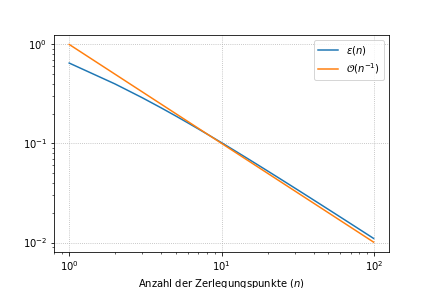
\includegraphics
  [width = 0.5 \textwidth]
  {Fehler zum Endzeitpunkt vs. Anzahl der Zerlegungspunkte}
  \caption{Konvergenzplot}
  \label{Konvergenzplot}
\end{figure}

\end{solution}

\begin{exercise}

Seien $A, M \in \R^{n \times n}$ symmetrisch, positiv definit und $f \in C([0, T], \R^n)$. Weiter sei $y_{y_0} \in C^1([0, T], \R^n)$ Lösung des Anfangswertproblems

\begin{align*}
  M y^\prime(t) = -A y(t) + f(t),
  \quad
  t \in [0, T],
  \quad
  y(0) = y_0
\end{align*}

zu einem beliebigen $y_0 \in \R^n$.
Zeigen Sie elementar, dass $y_0 \mapsto y_{y_0}(t)$ für jedes $t \in [0, T]$ Lipschitzstetig mit Lipschitz-Konstante $1$ bezüglich der von $M$ induzierten Norm $\norm[M]{\cdot}: x \mapsto \sqrt{x^T M x}$ ist.
Ist das Problem in diesem Sinne gut konditioniert?

\end{exercise}

\begin{solution}

Trivial!

\end{solution}

\begin{exercise}

Sei $y \in C^1(\R_{\geq 0}, \R)$ Lösung des Anfangswertproblems

\begin{align*}
  y^\prime(t) = \lambda y(t),
  \quad
  t > 0,
  \quad
  y(0) = y_0
\end{align*}

mit einem $\lambda < 0$.
Sei $h > 0$ eine konstante Schrittweite, $t_j := jh$, $j \in \N_0$, und $y^e_j$ bzw. $y^i_j$ die Approximationen an $y(t_j)$ aus dem expliziten bzw. impliziten Eulerverfahren.
Untersuchen Sie in Abhängigkeit von $\lambda$ und $h$ das Verhalten von $y^e_j$ bzw. $y^i_j$ für $j \to \infty$ und vergleichen Sie es mit dem der exakten Lösung $y(t_j)$.

\end{exercise}

\begin{solution}

Das Anfangswertproblem kann durch $f(t, y) = \lambda y$ beschrieben werden. Man verifiziert unmittelbar, dass die exakte Lösung folgende ist.

\begin{align*}
  y(t) = e^{\lambda t} y_0
\end{align*}

Damit erhält man

\begin{align*}
  y(t_j) \xrightarrow{j \to \infty} 0.
\end{align*}

Die Approximationen $y_j^{\mathrm{e}}$ und $y_j^{\mathrm{i}}$ sollten also auch für $j \to \infty$ verschwinden. \\

Mit $j \in \N_0$ lautet die explizite Euler Methode

\begin{align*}
  \Phi(t_j, y_j^{\mathrm{e}}, h) := f(t_j, y_j^{\mathrm{e}}),
  \quad
  y_{j+1}^{\mathrm{e}} := y_j^{\mathrm{e}} + h \Phi(t_j, y_j^{\mathrm{e}}, h).
\end{align*}

Man erhält also konkret

\begin{align*}
  y_{j+1}^{\mathrm{e}}
  =
  y_j^{\mathrm{e}} + h \lambda y_j^{\mathrm{e}}
  =
  (1 + h \lambda) y_j^{\mathrm{e}}.
\end{align*}

Damit folgt unmittelbar

\begin{align*}
  y_j^{\mathrm{e}}
  =
  (1 + h \lambda)^j y_0.
\end{align*}

Dieser Ausdruck ist für $y_0 = 0$ offensichtlich konstant $0$ und somit dagegen konvergent.
Er verschwindet aber auch für $|1 + h \lambda| < 1$.
Sollte allerdings $y_0 \neq 0$ und $|1 + h \lambda| \geq 1$ so konvergiert er nicht.
Dabei oszilliert die Approximation um die $t$-Achse, wenn $1 + h \lambda < 0$.
Um das zu vermeiden, muss für gegebenes $\lambda < 0$, $h > 0$ hinreichend klein sein. \\

Mit $j \in \N_0$ lautet die implizite Euler Methode

\begin{align*}
  \Phi(t_j, y_j^{\mathrm{i}}, y_{j+1}^{\mathrm{i}}, h) := f(t_{j+1}, y_{j+1}^{\mathrm{i}}),
  \quad
  y_{j+1}^{\mathrm{i}} := y_j^{\mathrm{i}} + h \Phi(t_j, y_j^{\mathrm{i}}, y_{j+1}^{\mathrm{i}}, h).
\end{align*}

Man erhält also konkret

\begin{align*}
  y_{j+1}^{\mathrm{i}}
  =
  y_j^{\mathrm{i}} + h \lambda y_{j+1}^{\mathrm{i}}
  \Rightarrow
  y_{j+1}^{\mathrm{i}}
  =
  (1 - h \lambda)^{-1} y_j^{\mathrm{i}}.
\end{align*}

Damit folgt unmittelbar

\begin{align*}
  y_j^{\mathrm{i}}
  =
  (1 - h \lambda)^{-j} y_0.
\end{align*}

Dieser Ausdruck ist für $y_0 = 0$ offensichtlich konstant $0$ und somit dagegen konvergent.
Er verschwindet aber auch für

\begin{align*}
  |1 - h \lambda|^{-1} < 1
  \Leftrightarrow
  1 < |1 - \underbrace{h \lambda}_{< 0}| = 1 - h \lambda
  \Leftrightarrow
  h \lambda < 0.
\end{align*}

Wir erkennen also, dass bei diesem Anfangswertproblem die Approximation mit dem impliziten Eulerverfahren vorzuziehen ist, da
diese unter den gegebenen Voraussetzungen für $j \to \infty$ immer verschwindet. \\

Schließlich, konvergieren die Approximationen beider Eulerverfahren, für $h \to 0$, gegen die exakte Lösung.

\begin{align*}
  y_j^{\mathrm{e}}
  =
  \pbraces
  {
    (1 + h \lambda)^\frac{1}{h \lambda}
  }^{\lambda t_j}
  \xrightarrow{h \to 0}
  y(t_j),
  \quad
  y_j^{\mathrm{i}}
  =
  -\pbraces
  {
    (1 - h \lambda)^\frac{1}{h \lambda}
  }^{-\lambda t_j}
  \xrightarrow{h \to 0}
  y(t_j)
\end{align*}

\end{solution}

\begin{exercise}

Beweisen Sie folgende Variation des Satzes 1.3 aus der Vorlesung:
$f$ sei bezüglich des zweiten Argumentes nur einseitig Lipschitz-stetig, d.h. es existiert ein $L_+ \in \R$ mit

\begin{align*}
  \abraces{f(t, y) - f(t, z), y - z}
  \leq
  L_+ \norm[2]{y - z}^2,
  \quad
  (t, y), (t, z) \in J \times \Omega.
\end{align*}

Weiter sei auch $z$ eine Lösung der Differentialgleichung $z^\prime = f(t, z)$ (d.h. $\delta = 0$ in Satz 1.3). Dann gilt

\begin{align*}
  \norm[2]{y(t) - z(t)}
  \leq
  \norm[2]{y(t_0) - z(t_0)} e^{L_+ (t - t_0)},
  \quad
  t \geq t_0.
\end{align*}

\end{exercise}

\begin{solution}

Zuerst, bemerken wir, dass

\begin{align*}
  \frac{d}{d \tau} \norm[2]{y(\tau) - z(\tau)}^2
  & =
  \sum_{i=1}^n \frac{d}{d \tau} (y_i(\tau) - z_i(\tau))^2
  =
  \sum_{i=1}^n 2 (y_i(\tau) - z_i(\tau))(y_i^\prime(\tau) - z_i^\prime(\tau)) \\
  & =
  2 \abraces
  {
    y^\prime(\tau) - z^\prime(\tau),
    y(\tau) - z(\tau)
  }_2
  =
  2 \abraces
  {
    f(\tau, y(\tau)) - f(\tau, z(\tau)),
    y(\tau) - z(\tau)
  }_2
  \leq
  2 L_+ \norm[2]{y(\tau) - z(\tau)}^2.
\end{align*}

Aus dem Hauptsatz der Differnetial- und Integralrechnung, der Dreiecksungleichung, folgt also

\begin{align*}
  \norm[2]{y(t) - z(t)}^2
  & \leq
  \norm[2]{y(t_0) - z(t_0)}^2
  +
  \Int[t_0][t]
  {\frac{d}{d \tau} \norm[2]{y(\tau) - z(\tau)}^2}{\tau} \\
  & \leq
  \norm[2]{y(t_0) - z(t_0)}^2
  +
  2 L_+ \Int[t_0][t]
  {\norm[2]{y(\tau) - z(\tau)}^2}{\tau}.
\end{align*}

Mit dem Grönwall-Lemma, und den (jetzt nicht unmotivierten) Definitionen

\begin{align*}
  v(t) := \norm[2]{y(t) - z(t)}^2,
  \quad
  A := v(t_0),
  \quad
  B := 0,
\end{align*}

erhalten wir

\begin{align*}
  \norm[2]{y(t) - z(t)}^{2}
  \leq
  \norm[2]{y(t_0) - z(t_0)}^2 e^{2 L_+ (t - t_0)}.
\end{align*}

Wenn man hier noch die $\sqrt{\cdot}$ zieht, folgt die Behauptung.

\end{solution}

\begin{exercise}

Sei $A \in \R^{n \times n}$ symmetrisch und $y \in C^1([0, T], \R^n)$ Lösung des Anfangswertproblems

\begin{align*}
  y^\prime(t) = A y(t),
  \quad
  t \in [0, T],
  \quad
  y(0) = y_0.
\end{align*}

Berechnen Sie die Lipschitz-Konstante sowie die einseitige Lipschitz-Konstante der zugehörigen Funktion $f$ und vergleichen Sie die Aussage aus dem Satz 1.3 mit der Aussage aus Aufgabe 4.

Hinweis: Symmetrische Matrizen sind diagonalisierbar.

\end{exercise}

\begin{solution}

Die zugehörige Funktion ist $f: (t, y) \mapsto Ay$.
Also $\Forall (t, y), (t, z) \in \R \times \R^n:$

\begin{align*}
  \norm{f(t, y) - f(t, z)}
  =
  \norm{A (y - z)}
  \leq
  \norm{A} \cdot \norm{y - z}.
\end{align*}

Damit ist die Lipschitz-Konstante $L = \norm{A}$. \\

Weil $A$ diagonalisierbar ist, existiert eine Basis $B \in \R^{n \times n}$ aus Eigenvektoren von $A$, sodass $D := B^{-1} A B$ eine Diagonalmatrix ist.
$\rho(A) := \max \Bbraces{|\lambda|: \lambda \text{ Eigenwert von } A}$ ist der Spektralradius von $A$.
Weil $A = A^T$ symmetrisch ist, folgt $\Forall (t, y), (t, z) \in \R \times \R^n:$

\begin{align*}
  \abraces{f(t, y) - f(t, z), y - z}
  & =
  \abraces{A (y - z), y - z}
  =
  (y - z)^T A (y - z)
  =
  (y - z)^T B D B^{-1} (y - z) \\
  & \leq
  (y - z)^T B \rho(A) B^{-1} (y - z)
  =
  \rho(A) (y - z)^T (y - z)
  =
  \rho(A) \norm[2]{y - z}^2.
\end{align*}

Damit ist die einseitige Lipschitz-Konstante $L_+ = \rho(A)$. \\

Für jede natürliche Matrixnorm $\norm{\cdot}$ und jede Matrix $A \in \K^{n \times n}$, gilt $\rho(A) \leq \norm{A}$. Also ist die einseitige Lipschitz-Konstante \enquote{besser} also die Lipschitz-Konstante, d.h. $L_+ \leq L$. \\

Gemeinsam mit der Aufgabe 4, erhält man also dieselbe Konklusio, wie in Satz 1.3, mit $\delta = 0$, also einer exakten Lösung $z$.

\end{solution}


\end{document}
